\documentclass{article}
\usepackage{amsmath}
\usepackage{graphicx}
\usepackage{graphics}
\usepackage{amssymb}
\usepackage{booktabs}
\usepackage{listings}
\usepackage{color}
\usepackage{caption}
\usepackage{subcaption}
\usepackage[margin=2cm]{geometry}
\usepackage{epstopdf}

\begin{document}
\title{CS 5220 Project 3 Preliminary Report}
\author{Team 15 - Xiang Long (XL483), Yalcin Ozhabes (AO294), Bryce Evans (BAE43)}

\maketitle

\section{Introduction}

Our task is to profile and optimize an implementation of the all-pairs-shortest-paths algorithm that computes its result through repeated squaring of the minimum paths distance matrix. The parallelization of the implementation is done by OpenMP, and our task is to eventually produce another version using MPI instead. We have decided that for this report, we will profile and tune the current OpenMP version of the code, leaving the MPI implementation to be completed in the rest of the project.

\section{VTune Profiling}

We first profiled the given code using VTune Amplifier to discover hotspots in the code. Due to license limitations we were only able to profile the code on the Totient head node, but we believe similar results would have been obtained if we were able to perform profiling on the compute nodes. The relevant sections of the report is shown in Table~\ref{vtune}.

\begin{table}[h]
 \centering
  \begin{tabular}{ | l | r | r | r | r | }
 \hline
Function             & CPU Time &  CPU Time:Idle & CPU Time:Poor & CPU Time:Ideal \\ \hline
square               &  30.320s &             0s &        0.121s &        30.199s \\
gen\_graph            &   0.052s &         0.010s &        0.042s &             0s \\
fletcher16           &   0.030s &             0s &        0.030s &             0s \\
\_\_intel\_ssse3\_memcpy &   0.020s &             0s &        0.020s &             0s \\
genrand              &   0.019s &         0.010s &        0.009s &             0s \\
infinitize           &   0.009s &             0s &        0.009s &             0s \\ \hline
\end{tabular}
 \caption{VTune Report of Original Code}
 \label{vtune}
\end{table}

The results are for the default $2000 \times 2000$ matrix, and we have omitted columns that are all zeros and rows that are functions not part of path.c. It is clear that the vast majority of the time is taken by the square function, and that is where we should concentrate our optimization efforts.

\section{Scaling Studies of Original Code}

We also performed strong and weak scaling studies on the original code, and the performance varying with number of threads is shown in graphs of figures~\ref{strong-orig} and~\ref{weak-orig} respectively. Since the original code was parallelized using OpenMP, we expect some performance gains if more worker threads are available.

 \begin{figure}[h]
  \centering
  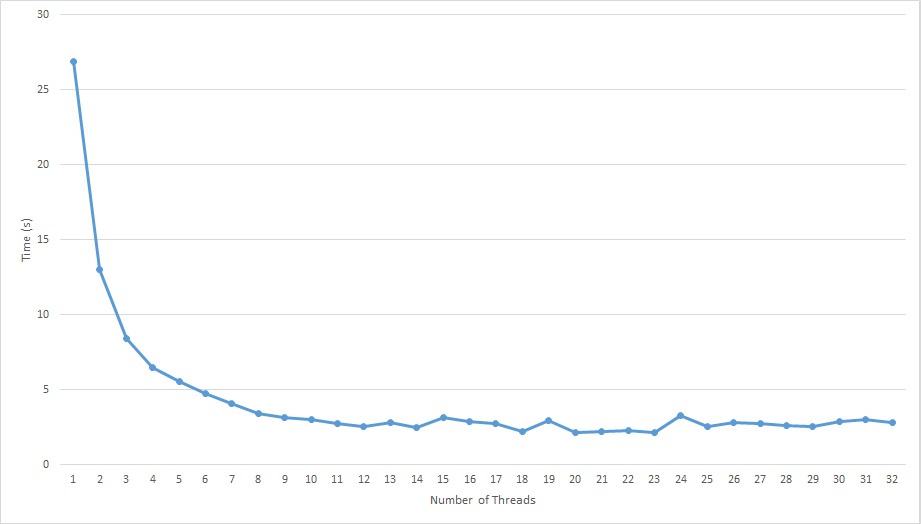
\includegraphics[width=0.7\linewidth]{strong-orig.png}
  \caption{Time taken for original algorithm on a fixed $2000 \times 2000$ matrix varying with number of threads}
  \label{strong-orig}
\end{figure}

 \begin{figure}[h]
  \centering
  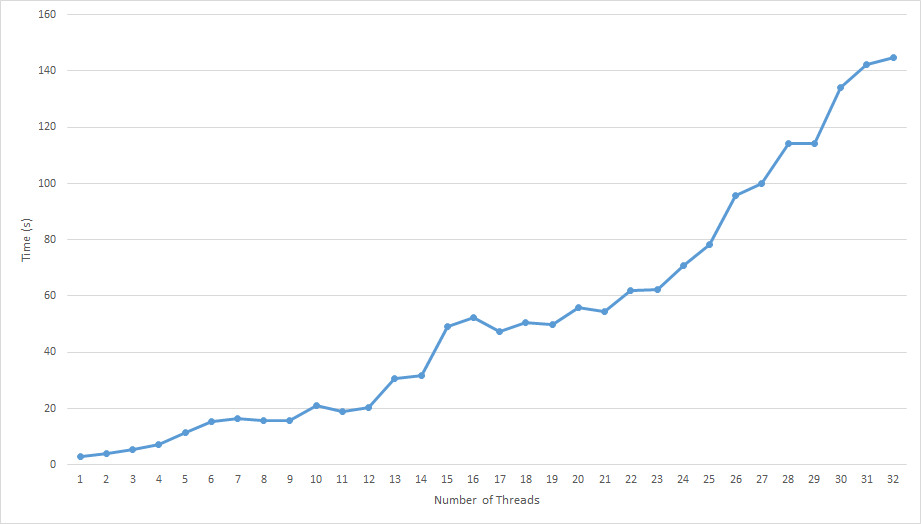
\includegraphics[width=0.7\linewidth]{weak-orig.png}
  \caption{Time taken for original algorithm on varying with number of threads with workload of each thread held constant}
  \label{weak-orig}
\end{figure}

In the strong scaling graph we can see that performance does improve if more worker threads are created, although there are diminishing returns and improvement is not significant after around 12 threads.

In the weak scaling study, we keep the workload of each thread constant as we increase the number of threads. This was done by starting with a $1000 \times 1000$ matrix initially, and multiplying the dimensions by the square root of the number of threads. Here we find that the time taken did not stay constant, which means the parallelization is optimal. With tuning and a better parallelized implementation we can hope to improve on this.

\section{Tuning}

The iteration order of this algorithm is exactly the same as matrix multiplication. Only difference is that we have one matrix and multiplying by its transpose. First step we take is to copy the transpose of the matrix into a separate array so that we get better locality. By doing so we were able to get approximately 4 times speed up. 

As a second step we divide the matrix into blocks to split up the work among the threads. We use almost exact copy of \texttt{dgemm\_blocked.c}. We change the array accesses to the first matrix as now we use the transposed copy of it. We also change the inner kernel and replace the multiplication with path length comparison and update.

The order of the \texttt{for} loops is such that every block of the resulting matrix is computed one by one. In other words, in the serial version, the outer loop iterates over the blocks of the resulting matrix so it does not go back to a previous block. This ordering is useful when we parallelize because we split up the work of the outer loop and each thread updates independent block of the result, reading the data from input matrices in a mixed order.

This blocking strategy worked well and we got up to 12x speed up. 

 \begin{figure}[h]
  \centering
  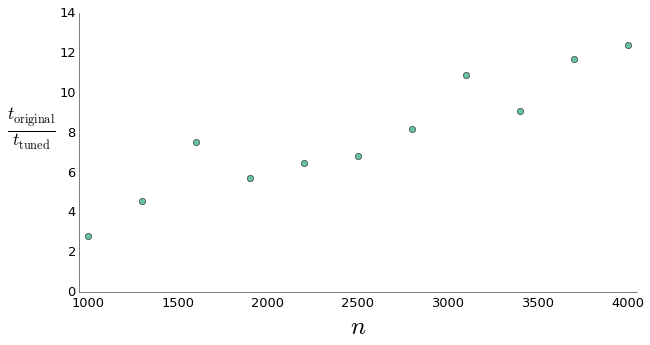
\includegraphics[width=0.7\linewidth]{tunedPerformance.png}
  \caption{Speed up by tuning the OpenMP implementation with blocked load partitioning.}
  \label{tunedPerformance}
\end{figure}

\section{Compiler Flags}
Given the similarity of the problem to Matrix Multiplication, we attempted to reuse many compiler flags from the previous assignment. These flags focus on vectorizing multiplications and fast loop unrolling, both of which are ideal for this algorithm. In addition to the flags provided, we added \texttt{-no-prec-div -ipo -unroll-aggressive}. These surprisingly resulted in worse performance, slowing down our program by 7\% on average. We did not find compiler flags that further increased our result times.

\section{MPI Implementation}
For our MPI implementation, we divide the workload for multiple compute nodes as follows. Each node is assigned a region of the matrix in the form of a column set to optimize, and all the nodes have the same copy of the whole matrix. The nodes independently find the best values for the elements within their assigned region based on its view of the matrix. Here thread-level parallelization are utilized to find the optimal values for multiple elements in the assigned region simultaneously. The finished regions from each node is then broadcasted to all other nodes. There is therefore a barrier at these points, where all nodes wait to receive updates from all other nodes before continuing to do the next iteration. 

\includegraphics[width=0.7\linewidth]{mpi-plot.PNG}

For working with MPI, we wanted to get a working version running quickly and so completed a simpler implementation that distributed the updates as columns to start. We believe that dividing the matrix into square blocks and using Cannon's Algorithm would have higher performance, though this implementation introduces many additional challenges. It has benefits because each node no longer has to store the entire matrix in memory, and so it would be superior for very large matrices that cannot fit entirely in memory. A downside is that broadcasts no longer are global, so while blocking is decreased,  a complex topology arises and each node no longer broadcasts, but sends a smaller packet to a subset of other nodes. In addition, Cannon's Algorithm requires square grids with is another downside of this method.





\end{document}
